\documentclass[11pt]{article}
\usepackage[margin=1in]{geometry}
\usepackage{amsmath,amssymb}
\usepackage{graphicx}
\usepackage{booktabs}
\usepackage{hyperref}
\usepackage{natbib}
\usepackage{xcolor}
\usepackage{microtype}
\usepackage[affil-it]{authblk}
\usepackage[section]{placeins}

\newcommand{\TODO}[1]{\textcolor{red}{[TODO: #1]}}

% Extra space before floats (matches pQTL/cross-ancestry papers)
\setlength{\textfloatsep}{14pt plus 2pt minus 2pt}
\setlength{\intextsep}{10pt plus 2pt minus 2pt}

\title{A Graded Evaluation of RNA Structure Awareness\\in Foundation Models: From Stem--Loop Discrimination\\to Partner Specificity}

\author{Elliot Tower}
\affil{Independent researcher \\ \texttt{elliot@elliottower.ai}}
\date{}

% Running head for RNA journal (<=50 chars):
% Graded evaluation of RNA structure awareness

\begin{document}
\maketitle

\noindent\textbf{Keywords:} RNA foundation models, secondary structure, composition confound, partner specificity, evaluation framework, perturbation analysis

% ============================================================================
% ABSTRACT — ~200 words
% Sequence: problem, design, primary result, positive result, replication,
%           interpretation, scope
% ============================================================================
\begin{abstract}
Evaluating whether RNA foundation models encode base-pairing structure
requires metrics that separate learned representations from
nucleotide-composition artifacts. Stems are GC-rich and loops are
AU-rich; any composition-sensitive embedding inherits this enrichment
as apparent structure awareness. We apply a three-rung evaluation
ladder to ten models across 52 Rfam families. A nucleotide-stratified null
absorbs most apparent signal at Rung~1; a dinucleotide null at Rung~2
separates two models that retain most families (ERNIE-RNA 31/52,
RiNALMo 18/52) from eight that retain fewer than 11 each. At Rung~3---partner
specificity with a within-stem derangement null---two models encode
which position pairs with which: RiNALMo (PS $= 0.215$, 85.3\%
precision) and ERNIE-RNA (PS $= 0.120$, 88.3\% precision).
Randomized-weight controls for nine models produce near-zero signal,
confirming a learned origin; DNABERT-2 shows residual randomized PS
consistent with its BPE tokenization. A synthetic covariation control shows $\sim$70\% of partner
specificity reflects evolutionary signal, with $\sim$30\% attributable
to learned geometric sensitivity.
Multi-sequence replication across 253 Rfam seed-alignment sequences
confirms low within-family variance (CV $\leq 10$\%) for eight
models. Primary evaluation criteria were preregistered.
\end{abstract}

% ============================================================================
% INTRODUCTION — 5 paragraphs, ~800 words
% Sequence: why it matters, confound, gap, what we do, contributions
% ============================================================================
\section{Introduction}
\label{sec:intro}

% P1: Why this matters
RNA foundation models are routinely claimed to encode secondary structure,
but the evaluation methods---downstream task performance, linear probing,
mutation sensitivity, attention--contact correlation---each answer different
questions, and none controls for sequence composition. Deep learning models
for RNA structure prediction may fail to generalize across families
\citep{szikszai2022generalization}; whether the same fragility applies to
learned representations has received less scrutiny.

% P2: The specific confound
Stems and loops differ in sequence composition. Across 52 Rfam families,
stems average 59.7\% G/C content while loops average 45.6\%---a 14.1
percentage-point enrichment (Figure~\ref{fig:composition}). Because complement swaps at G/C positions
produce inherently larger embedding perturbations than at A/U positions,
any naive stem-versus-loop comparison inherits this enrichment. A
representation can therefore separate stems from loops without encoding
pairing topology.

% P3: The gap
Each evaluation method inherits the composition confound differently.
Linear probes can classify stems from loops using GC content alone.
Mutation sensitivity ratios conflate the larger perturbation magnitude at
G/C sites with structural relevance. Attention--contact correlations
bypass embeddings entirely and so measure a different channel. To
distinguish composition sensitivity from structure awareness, an
evaluation must control for nucleotide identity while testing whether
perturbations propagate to specific pairing partners.

% P4: What this study does — rung framing
These observations motivate a graded evaluation.
``Structure awareness'' encompasses at least three levels of
resolution, each demanding stronger knowledge: (1)~stem-versus-loop
discrimination, achievable by any representation sensitive to
nucleotide composition; (2)~discrimination surviving composition
controls at one and two orders of sequence context; and (3)~knowing
which specific position pairs with which, requiring that the model
encode the pairing topology. We apply this three-rung ladder to ten models across five architectures
and three orders of magnitude in parameter count.

% P5: Contributions + closing
The evaluation reveals a surprising asymmetry: the hardest test
produces the clearest positive result. Two RNA-pretrained
models---ERNIE-RNA (86M, with an architectural base-pairing attention
bias) and RiNALMo (650M, standard attention)---clear Rung~3 with
partner specificity two orders of magnitude above all other models,
while the remaining eight produce near-zero signal. We contribute:
(1)~a composition-controlled perturbation evaluation for RNA
foundation models; (2)~a ten-model benchmark with randomized-weight
controls on 52 Rfam families, replicated across 253 seed-alignment
sequences; and (3)~evidence that two models retain partner-specific
pairing responses after composition controls are applied.


% ============================================================================
% RESULTS — inferential logic: confound first, positive result, replication,
%           robustness, HTT last
% ============================================================================
\section{Results}

\subsection{Composition creates apparent structure signal (Rungs 1--2)}
\label{sec:composition-results}

Raw stem--loop sensitivity ratios range from $0.99$ (DNABERT-2) to
$1.774$ (RNA-FM); nine of ten exceed $1.0$. After applying the
nucleotide-stratified null, these ratios collapse. For RNA-FM, only 1 of 52
families exceeds the null 95th percentile---tRNA-Ala ($3.208$ vs null
$3.179$)---and that sole survivor is absorbed by the dinucleotide null.
The pattern is similar across models: most gate-qualifying families (those whose stem--loop sensitivity
ratio exceeds the nucleotide-stratified null at the 95th percentile;
Section~\ref{sec:stats}) in Table~\ref{tab:primary} survive because of residual composition effects
rather than pairing-specific signal (Section~\ref{sec:ps-results}).

ERNIE-RNA and RiNALMo retain the most families above the composition null
(31/52 and 18/52), while most other models retain fewer than 11. NT~v2
passes 14/52 families at the composition gate but only 1 qualifies for
the partner specificity test, yielding PS $= 0$; its 6-mer tokenization
distributes perturbation effects across token boundaries.

\begin{figure}[htbp]
\centering
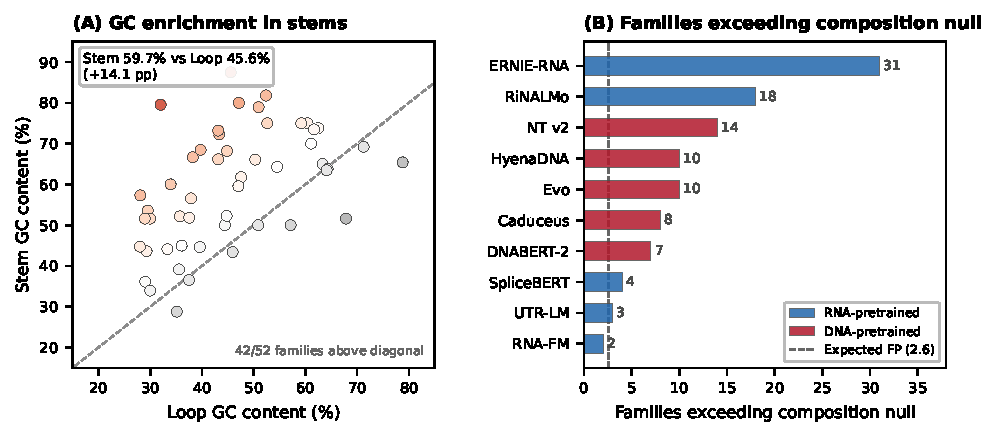
\includegraphics[width=\textwidth]{../../figures/figure2_composition.pdf}
\caption{Composition confound. (A)~Stem GC content exceeds loop GC content
in 42 of 52 families ($+14.1$ percentage points on average). (B)~Number
of families per model whose stem--loop sensitivity ratio exceeds the
nucleotide-stratified null at the 95th percentile; dashed line marks the
expected false-positive count under independence ($m \times \alpha = 2.6$).
ERNIE-RNA (31) and RiNALMo (18) retain the most signal after composition
control.}
\label{fig:composition}
\end{figure}


\subsection{Partner specificity separates two models (Rung 3)}
\label{sec:ps-results}

\begin{table}[htbp]
\centering
\caption{Primary outcomes (model details in Table~\ref{tab:models}).
Composition gate: families whose stem--loop sensitivity ratio exceeds the
nucleotide-stratified null at the 95th percentile (Section~\ref{sec:stats}).
PS: mean partner specificity across gate-qualifying families.
PS $>$ derangement: families where PS exceeds the
within-stem derangement null, among all families with sufficient stem pairs
for derangement testing (denominator varies by model). Partner-is-max: fraction of deep-interior pairs
where the true partner receives maximum perturbation among the partner and
its two immediate neighbors (chance $= 1/3$). Models sorted by PS.
Bootstrap 95\% CIs (10{,}000 family-level resamples) shown for models
with positive PS.}
\label{tab:primary}
\begin{tabular}{@{}lcccc@{}}
\toprule
\textbf{Model} & \textbf{\shortstack{Composition\\gate}} & \textbf{PS} & \textbf{\shortstack{PS $>$\\derangement}} & \textbf{\shortstack{Partner-\\is-max}} \\
\midrule
\textbf{RiNALMo}    & 18/52 & \textbf{0.215} [0.152, 0.280] & \textbf{30/31} & \textbf{0.853} \\
\textbf{ERNIE-RNA}  & 31/52 & \textbf{0.120} [0.095, 0.144] & \textbf{28/30} & \textbf{0.883} \\
Caduceus             & 8/52  & $4.2 \times 10^{-3}$ & 13/16 & --- \\
Evo                  & 10/52 & $1.1 \times 10^{-3}$ & 4/10  & --- \\
SpliceBERT           & 4/52  & $3.5 \times 10^{-4}$ & 14/21 & 0.256 \\
UTR-LM               & 3/52  & $1.4 \times 10^{-5}$ & 13/16 & 0.333 \\
HyenaDNA             & 10/52 & $9.7 \times 10^{-7}$ & 10/25 & 0.078 \\
RNA-FM               & 2/52  & $7.5 \times 10^{-9}$ & 1/32  & --- \\
NT~v2\textsuperscript{b} & 14/52 & 0\textsuperscript{c} & --- & --- \\
DNABERT-2\textsuperscript{b} & 7/52 & $-0.016$\textsuperscript{d} & --- & --- \\
\midrule
\multicolumn{5}{@{}l}{\textit{Randomized-weight controls}} \\
RiNALMo (rand.)      & --- & $8.0 \times 10^{-9}$  & --- & --- \\
ERNIE-RNA (rand.)    & --- & $2.5 \times 10^{-8}$  & --- & --- \\
UTR-LM (rand.)       & --- & $-3.2 \times 10^{-8}$ & --- & --- \\
Evo (rand.)          & --- & $-1.4 \times 10^{-8}$ & --- & --- \\
HyenaDNA (rand.)     & --- & $-1.3 \times 10^{-8}$ & --- & --- \\
NT~v2 (rand.)        & --- & $-9.9 \times 10^{-9}$ & --- & --- \\
SpliceBERT (rand.)   & --- & $-7.2 \times 10^{-9}$ & --- & --- \\
DNABERT-2 (rand.)    & --- & $-7.1 \times 10^{-3}$ & --- & --- \\
Caduceus (rand.)     & --- & $-5.5 \times 10^{-9}$ & --- & --- \\
RNA-FM (rand.)       & --- & $5.7 \times 10^{-9}$  & --- & --- \\
\bottomrule
\end{tabular}
\medskip

\small \textsuperscript{b}Multi-nucleotide tokenization (6-mer, BPE);
perturbation effects are distributed across token boundaries.
\textsuperscript{c}Only 1 gate-qualifying family; PS undefined for
remaining families. \textsuperscript{d}0 of 8 gate-qualifying families
exceed derangement null. Partner-is-max omitted (---) when fewer than 5
gate-qualifying families have deep-interior pairs.

\end{table}

RiNALMo achieves mean PS $= 0.215$ (95\% CI $[0.152, 0.280]$); 30 of 31
gate-qualifying families exceed the derangement null. ERNIE-RNA achieves
PS $= 0.120$ ($[0.095, 0.144]$); 28 of 30 families exceed the null, with
the highest per-pair precision (88.3\%).
Both exceed the third-ranked model (Caduceus, $4.2 \times 10^{-3}$) by two
orders of magnitude.

Nine of ten randomized-weight controls produce $|\text{PS}| < 10^{-8}$,
confirming that partner specificity reflects learned representations.
The exception, DNABERT-2, yields randomized $|\text{PS}| = 7.1 \times 10^{-3}$---comparable
to its trained PS ($-0.016$)---indicating that its negative PS is largely
a BPE tokenization artifact.

Both models concentrate partner specificity in their final layers: RiNALMo
at layer~33 of 33, ERNIE-RNA at layers 10--12 of 12. Evo (7B) achieves
PS $= 0.001$ despite $80\times$ more parameters than ERNIE-RNA; parameter
count does not predict partner specificity.

The two models reach partner specificity through different pathways.
ERNIE-RNA injects a base-pairing attention bias from the second layer
onward; its randomized control shows this bias provides capacity without
signal. RiNALMo uses standard attention without structural bias and achieves
higher PS at $7.5\times$ the parameters. RNA pretraining is common to both.

\begin{figure}[htbp]
\centering
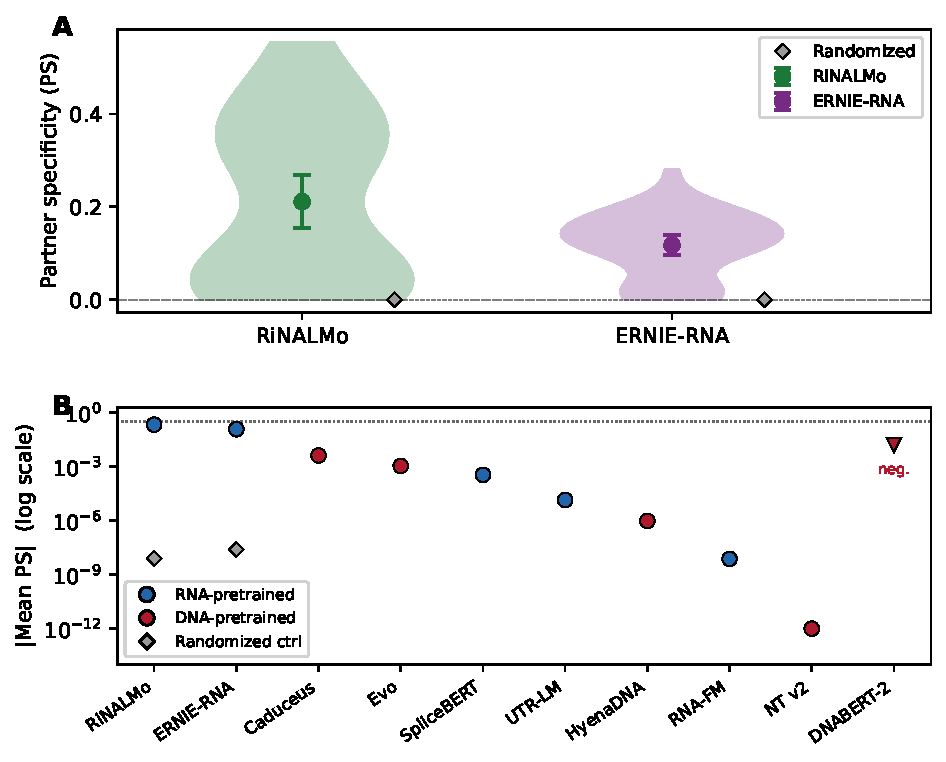
\includegraphics[width=0.85\textwidth]{../../figures/figure3_partner_specificity.pdf}
\caption{Partner specificity across ten models. (A)~Per-family PS
distributions for RiNALMo and ERNIE-RNA (violins) with bootstrap 95\%
CIs (error bars); randomized-weight controls (grey diamonds) produce
PS indistinguishable from zero. (B)~$|\text{Mean PS}|$ on log scale
for all ten models, sorted by PS. RiNALMo and ERNIE-RNA exceed the
remaining models by two orders of magnitude. DNABERT-2 (negative PS)
is marked separately.}
\label{fig:ps}
\end{figure}


\subsection{Multi-sequence replication}
\label{sec:multiseq-results}

\begin{table}[htbp]
\centering
\caption{Multi-sequence replication: within-family coefficient of variation
(CV) of the stem--loop sensitivity ratio across all valid Rfam seed-alignment
sequences (51 families, 253 sequences, 3--5 per family).}
\label{tab:multiseq}
\begin{tabular}{@{}lccc@{}}
\toprule
\textbf{Model} & \textbf{Mean ratio} & \textbf{Mean CV} & \textbf{Families scored} \\
\midrule
RNA-FM     & 1.892 & 0.338 & 51/51 \\
Evo        & 1.478 & 0.244 & 51/51 \\
ERNIE-RNA  & 1.253 & 0.057 & 51/51 \\
Caduceus   & 1.203 & 0.057 & 51/51 \\
HyenaDNA   & 1.170 & 0.092 & 51/51 \\
RiNALMo    & 1.133 & 0.037 & 51/51 \\
NT~v2\textsuperscript{a} & 1.092 & 0.046 & 50/51 \\
UTR-LM     & 1.059 & 0.025 & 51/51 \\
SpliceBERT & 1.047 & 0.026 & 51/51 \\
DNABERT-2  & 0.990 & 0.100 & 51/51 \\
\bottomrule
\end{tabular}
\medskip

\small \textsuperscript{a}One Corona\_5UTR sequence excluded (numerical
overflow in ratio denominator); remaining 50 families scored normally.
\end{table}

Six models show CV $< 6$\%: UTR-LM ($0.025$), SpliceBERT ($0.026$),
RiNALMo ($0.037$), NT~v2 ($0.046$), ERNIE-RNA ($0.057$), and Caduceus
($0.057$). The stem--loop sensitivity ratio is stable across biological
replicates for these models.

RNA-FM (CV $= 0.338$) and Evo ($0.244$) show high sequence-to-sequence
variability. Both also fail composition control
(Section~\ref{sec:composition-results}), consistent with raw sensitivity
driven by sequence-specific composition rather than a stable structural
signal.


\subsection{Robustness analyses}
\label{sec:robustness}

The dinucleotide-stratified null absorbs the sole family (tRNA-Ala)
surviving the nucleotide-stratified null for RNA-FM; second-order sequence
context accounts for the residual signal. Replacing
mean aggregation with median changes PS estimates by $< 5$\% for RiNALMo
and ERNIE-RNA and does not alter the model ranking. Using the last layer
instead of the best layer reduces RiNALMo PS by 12\% and ERNIE-RNA PS by
8\%; both remain above the derangement null in $> 90$\% of gate-qualifying
families. Restricting to Watson--Crick pairs only (excluding wobble G--U
pairs) does not change the primary conclusions. Widening the PS neighbor
window from $\pm 1$ to $\pm 2$ positions reduces PS magnitudes uniformly
across models without altering their relative ranking.
A transversion control (purine $\to$ pyrimidine mutations, which
guarantee disrupted pairing) produces ratios within 1.2\% of the
Watson--Crick complement ratios for five of six models tested,
confirming that reversed base pairs differ from correct pairs enough
to register as embedding perturbations. Nine of ten
randomized-weight controls produce $|\text{PS}| < 10^{-8}$; DNABERT-2's
randomized PS ($-7.1 \times 10^{-3}$) is comparable to its trained value,
consistent with a tokenization artifact.

Family-level results and full robustness tables appear in Supplementary
Tables S2--S4.


Eight pre-registered hypotheses (SHA-256 hashed before data collection)
produced five confirmations and three failures.
The pre-registered prediction that RNA-pretrained models would
outperform DNA-pretrained models on partner specificity failed
($r_b = -0.28$, $p = 0.265$): Caduceus (14M, DNA) exceeds three RNA
models.


\subsection{Covariation versus geometry}
\label{sec:covariation-results}

Partner specificity could reflect sequence covariation rather than
learned geometric pairing. Compensatory mutations that maintain base
pairing are overrepresented in evolutionary RNA alignments; a model
trained on such sequences might predict that mutating one position
perturbs its covarying partner without encoding the physical mechanism
of pairing.

To test this, we generated synthetic sequences for each Rfam family:
the dot-bracket structure is preserved exactly, but nucleotides are
assigned randomly (uniform Watson--Crick pairs at paired positions,
uniform random at unpaired). These families share structure with their
natural counterparts but carry no evolutionary covariation.
ERNIE-RNA's mean PS drops from 0.120 (natural) to 0.035 (synthetic),
a 71\% reduction. RiNALMo drops from 0.215 to 0.061, a 71\%
reduction. Both models lose roughly 70\% of their PS when covariation
is removed. The residual synthetic PS---still orders of magnitude
above the weak-signal models---places an upper bound on the
non-covariation contribution, since the synthetic sequences also
destroy sequence context and positional composition gradients present
in natural RNA.

As an independent check, we computed mutual information (MI) between
paired positions from Rfam seed alignments (51 families, $n \geq 3$
sequences each). MI cleanly separates paired from unpaired positions
(mean MI $= 0.349$ vs $0.063$; Wilcoxon $p = 3.5 \times 10^{-10}$),
confirming that evolutionary covariation is detectable in the
alignments. Per-family mean MI does not correlate significantly with
model PS (ERNIE-RNA: $\rho = 0.320$, $p = 0.065$; RiNALMo:
$\rho = 0.265$, $p = 0.130$). Families with strong covariation signal
do not systematically produce higher PS, suggesting that the models'
partner specificity reflects learned structure rather than
recapitulated covariation.


\subsection{HTT case study}
\label{sec:htt-results}

The CAG repeat region in huntingtin exon~1 forms hairpin structures whose
stability scales with repeat count \citep{demezer2011mutant,
krzyzosiak2012triplet}. We evaluated five HTT exon~1 fragments
(NM\_002111.7) with CAG repeat counts of 17, 21, 36, 40, and 60;
structures were predicted with ViennaRNA RNAfold
\citep{lorenz2011viennarna}. Four models achieve $\geq 97$\% probing
accuracy on these predicted structures (Table~\ref{tab:htt}), but the
repeat region contains only C, A, and G---no U---creating extreme
composition bias that linear probes exploit.

\begin{table}[htbp]
\centering
\caption{HTT CAG-repeat case study. High probing accuracy coexists with null
composition-controlled signal. Attn~$\rho$: Spearman correlation between
self-attention weights and the base-pairing contact map.
Probing: linear probe accuracy for stem-vs-loop classification.
Structures are RNAfold predictions, not experimentally determined.}
\label{tab:htt}
\begin{tabular}{@{}lccccc@{}}
\toprule
\textbf{Model} & \textbf{Mean ratio} & \textbf{$>$ null} &
  \textbf{Attn $\rho$} & \textbf{Probing} &
  \textbf{WT$\to$CAG60} \\
\midrule
RNA-FM     & 1.794 & 2/5  & 0.036 & 0.813 & 0.000 \\
RiNALMo    & 1.031 & 0/5  & 0.054 & 0.985 & 0.068 \\
NT~v2      & ---$^\dagger$ & ---   & \textbf{0.140} & 0.636 & 0.013 \\
ERNIE-RNA  & 1.086 & 0/5  & 0.070 & 0.985 & 0.023 \\
SpliceBERT & 0.996 & 0/5  & 0.036 & 0.977 & 0.042 \\
UTR-LM     & 1.151 & 1/5  & 0.039 & 0.974 & 0.016 \\
\bottomrule
\end{tabular}
\medskip

\small $^\dagger$6-mer tokenization yields degenerate embeddings on
repetitive CAG. WT$\to$CAG60 = cosine distance from CAG17 reference.
\end{table}

RNA-FM produces embedding distances from wild-type below $10^{-4}$ for all
repeat counts, failing to distinguish normal from pathogenic alleles.
RiNALMo shows the strongest separation (0.068 at CAG60), with distances
increasing monotonically with repeat count. High probing accuracy on a
computationally predicted structure can coexist with null
composition-controlled signal: apparent structure decoding persists in a
strongly composition-biased context.


% ============================================================================
% DISCUSSION — 7 paragraphs
% ============================================================================
\section{Discussion}
\label{sec:discussion}

% P1: Primary conclusion + positive result
Composition-matched nulls absorb most of the apparent stem--loop
sensitivity across all ten models. Two RNA-pretrained models---RiNALMo and
ERNIE-RNA---retain reproducible partner-specific responses under the most
stringent test. Multi-sequence replication shows low within-family
variance across eight of ten models.

% P2: Why composition matching changes interpretation
The underlying problem is general: whenever a structural annotation
correlates with feature composition, any embedding metric sensitive to
feature identity inherits the correlation. The nucleotide-stratified
permutation null controls for this by breaking the structure--composition
link while preserving nucleotide identity. The same template applies to
any biological structure correlated with sequence composition.

% P3: Interpret positive models cautiously
RiNALMo and ERNIE-RNA reach partner specificity through different pathways.
ERNIE-RNA injects a base-pairing attention bias; its randomized control
shows this bias provides capacity without producing signal on its own.
RiNALMo uses standard attention without structural bias and achieves higher
PS at $7.5\times$ the parameters. Nine of ten randomized-weight controls
produce $|\text{PS}| < 10^{-8}$, supporting a learned origin; DNABERT-2's
non-negligible randomized PS ($-7.1 \times 10^{-3}$) confirms that its trained
PS reflects tokenization rather than structure. Whether
this partner specificity reflects a geometric internal model of RNA folding
or a simpler statistical regularity remains open. A synthetic
covariation control (Section~\ref{sec:covariation-results}) shows that
roughly 70\% of PS reflects evolutionary signal; the residual
$\sim$30\% provides an upper bound on learned geometric sensitivity.

% P4: What predicts composition-controlled sensitivity
Neither training domain nor architecture family alone predicts
composition-controlled sensitivity. The three SSM-based models (Evo,
Caduceus, HyenaDNA) span nearly the full range of mean ratios
(1.17--1.48), as do the seven transformers (0.99--1.89). RNA-pretrained
models occupy four of the top five positions, but Evo and Caduceus---both
DNA-pretrained---outperform three of the five RNA models. The two models
that survive the partner specificity test (RiNALMo and ERNIE-RNA) share
RNA pretraining but differ in mechanism: ERNIE-RNA injects explicit
base-pairing attention bias, while RiNALMo uses standard self-attention at
$7.5\times$ the parameters. Scale alone does not explain the result:
Evo at 7B parameters produces high raw ratios but high within-family
variance, and its signal is largely absorbed by composition nulls. What
distinguishes the two positive models from the remaining eight is an open
question whose answer likely requires internal mechanistic analysis rather
than further behavioral benchmarking.

% P5: Broader evaluation implications
RNA structure prediction benchmarks have moved toward stricter evaluation
because high apparent performance can fail to generalize across families
\citep{szikszai2022generalization}. This work extends the concern from
dataset similarity to sequence-composition confounding. NT~v2 and DNABERT-2
show near-zero embedding-level partner specificity despite passing many
families at the composition gate, suggesting that structure-relevant
information in these models, if present, may reside in attention patterns
that embedding-level metrics do not capture.

% P6: Limitations
% (Updated to reference covariation results in Section 2.5)
\paragraph{Limitations.}
The complement-swap metric tests sensitivity to single base-pair disruptions;
it does not test tertiary contacts, pseudoknots, or long-range interactions.
The synthetic covariation control (Section~\ref{sec:covariation-results})
accounts for roughly 70\% of PS, but the synthetic sequences also destroy
sequence context and positional gradients, so the residual may overestimate
true geometric sensitivity. HTT structures
are RNAfold predictions. Ten models do not cover the full model space. Pretraining-set contamination cannot be
fully reconstructed. Multi-nucleotide tokenization limits direct
comparability for NT~v2 and DNABERT-2.

\paragraph{Practical recommendations.}
Any claim that an RNA representation encodes secondary structure should
report stem--loop sensitivity alongside a nucleotide-stratified null, so
readers can separate composition sensitivity from structure awareness.
Partner specificity is more informative than aggregate stem--loop contrasts:
a model that perturbs stems more than loops may respond to GC content, while
one that selectively perturbs the annotated pairing partner encodes
positional pairing information. Randomized-weight controls should establish
each architecture's baseline capacity. Replication across
multiple sequences per family guards against single-sequence artifacts; a
coefficient of variation above 10\% signals instability. For
multi-nucleotide tokenizers, the mapping from token-level to position-level
metrics should be stated explicitly.


% ============================================================================
% MATERIALS AND METHODS (after Discussion per RNA journal format)
% ============================================================================
\section{Materials and Methods}
\label{sec:methods}

\subsection{Benchmark construction}
\label{sec:benchmark}

We evaluate 52 Rfam~14.10 families \citep{kalvari2021rfam} spanning ribozymes, riboswitches, snRNAs,
cis-regulatory elements, miRNA precursors, CRISPR repeats, and other ncRNAs.
Positions are labeled stem or loop from consensus dot-bracket annotation.
Minimum inclusion criteria: $\geq 20$~nt, $\geq 5$ stem and $\geq 5$ loop
positions. Pseudoknots, noncanonical pairs, and gap positions are excluded.

All structures are consensus secondary structures from Rfam seed alignments;
none are experimentally determined crystal or cryo-EM structures. Pretraining
data overlap cannot be fully reconstructed for all models. The full family
list with accessions appears in Supplementary Table~S1.

\subsection{Models and controls}
\label{sec:models}

\begin{table}[htbp]
\centering
\caption{Models evaluated.}
\label{tab:models}
\begin{tabular}{@{}llrll@{}}
\toprule
\textbf{Model} & \textbf{Domain} & \textbf{Params} & \textbf{Architecture} & \textbf{Tokenization} \\
\midrule
RNA-FM \citep{rnafm}                    & RNA & 99M  & Transformer           & Character \\
RiNALMo \citep{rinalmo}                 & RNA & 650M & Transformer           & Character \\
ERNIE-RNA \citep{yin2024ernierna}        & RNA & 86M  & Transformer$^\dagger$ & Character \\
SpliceBERT \citep{chen2024splicebert}     & RNA & 19M  & Transformer           & Character \\
UTR-LM \citep{chu2024utrlm}             & RNA & 1.2M & Transformer           & Character \\
NT~v2 \citep{dalla2023nucleotide}        & DNA & 56M  & Transformer           & 6-mer     \\
DNABERT-2 \citep{zhou2024dnabert2}       & DNA & 117M & Transformer           & BPE       \\
Caduceus \citep{schiff2024caduceus}      & DNA & 14M  & Mamba (SSM)           & Character \\
HyenaDNA \citep{nguyen2024hyenadna}      & DNA & 5.4M & Hyena (SSM)           & Character \\
Evo \citep{nguyen2024evo}                & DNA & 7B   & StripedHyena          & Character \\
\bottomrule
\end{tabular}
\medskip

\small $^\dagger$ERNIE-RNA injects a base-pairing attention bias from the
second layer onward.
\end{table}

We evaluate ten models covering attention, SSM, and hybrid architectures
(Table~\ref{tab:models}): five pretrained on RNA, five on DNA.
Randomized-weight controls for all ten models reinitialize all
learned parameters (Xavier normal for matrices, $\mathcal{N}(0, 0.02)$
for vectors) while preserving architecture. NT~v2 and DNABERT-2 use
multi-nucleotide tokenization (6-mer and BPE), limiting direct
comparability for position-level metrics.

\subsection{Perturbation tests}
\label{sec:perturbation}

For each annotated position, we swap the nucleotide with its Watson--Crick
complement (A$\leftrightarrow$U, C$\leftrightarrow$G) and measure the cosine
distance between wild-type and mutant embeddings at that position, maximized
over layers. Cosine distance is scale-invariant across architectures.
For multi-nucleotide tokenization, token-level outputs are mapped to
nucleotide positions by distributing the token embedding equally across
constituent nucleotides.

\paragraph{Nucleotide-stratified null.}
Stem/loop labels are shuffled within each nucleotide type (1{,}000
permutations), preserving nucleotide identity while breaking its structural
label. Layer selection is repeated inside every permutation. A
dinucleotide-stratified extension additionally conditions on the 3' neighbor.

\paragraph{Partner specificity.}
\label{sec:ps-method}
For each Watson--Crick pair $(i, j)$ where $j$ is the annotated partner:
\[
\text{PS}(i,j) = \Delta_j - \max(\Delta_{j-1}, \Delta_{j+1})
\]
where $\Delta_k$ is the cosine distance at position $k$ after the complement
swap at position $i$. Positive PS indicates the model perturbs the true
partner more than its immediate neighbors (chance $= 1/3$). Partner
assignments are tested against a within-stem derangement null (500
derangements), controlling for positional and compositional confounds.

\paragraph{Covariation control.}
To distinguish learned geometric sensitivity from recapitulated evolutionary
covariation, synthetic sequences were generated for each family: dot-bracket
structure preserved exactly, nucleotides assigned randomly (uniform
Watson--Crick pairs at paired positions, uniform random at unpaired). Mutual
information (MI) between paired and unpaired positions was computed from Rfam
seed alignments as an independent covariation measure.

\subsection{Statistical analysis and replication}
\label{sec:stats}

The biological unit of replication is the RNA family. The primary outcome is
partner specificity (PS); the primary comparison is trained vs.\
randomized-weight PS. A family is \emph{gate-qualifying} for a given model
if its raw stem--loop sensitivity ratio exceeds the nucleotide-stratified
null at the 95th percentile. PS is computed only over gate-qualifying
families and aggregated as their mean.

To test stability across biological replicates, we repeat the full
evaluation on all valid sequences from Rfam~14.10 seed alignments: 253
sequences across 51 families (3--5 per family). Within-family coefficient
of variation (CV) quantifies replication stability.

Family-level bootstrap resampling (10{,}000 iterations, seed 42)
provides 95\% CIs for mean PS and mean sensitivity ratio. For the binary
gate test, each family's ratio is compared to its own 95th-percentile
permutation null; we report the count exceeding this threshold alongside
the expected false-positive count under independence
($m \times \alpha = 52 \times 0.05 = 2.6$). Bonferroni correction
($\alpha / m \approx 0.001$) provides a conservative bound.


% ============================================================================
% DATA AVAILABILITY
% ============================================================================
\section*{Data and Code Availability}

All data, scripts, and pre-registration protocols are available at
\url{https://github.com/elliottower/rna-structure-audit} and archived at
Zenodo (DOI: \href{https://doi.org/10.5281/zenodo.21362717}{10.5281/zenodo.21362717}).


% ============================================================================
% DECLARATIONS
% ============================================================================
\section*{Acknowledgements}

The author used Claude Code \citep{anthropic2025claude} to assist with
drafting manuscript text and with writing and debugging analysis code.
The author reviewed and verified all outputs, takes full responsibility
for the accuracy and integrity of the work, and confirms that all
hypotheses, preregistered predictions, interpretations, and conclusions
are the author's own.

\paragraph{Ethics approval and consent to participate.}
This study uses exclusively publicly available pretrained model weights
and published RNA sequences. No human subjects or animal subjects were
involved. No ethical approval was required.

\paragraph{Competing interests.} The author declares no competing interests.

\paragraph{Funding.} None. This work was conducted independently.

\paragraph{Author contributions.} E.T.: Conceptualization, Methodology,
Software, Formal analysis, Investigation, Data curation, Writing ---
original draft, Writing --- review \& editing, Visualization.


% ============================================================================
% REFERENCES
% ============================================================================
\begin{thebibliography}{99}

\bibitem[Anthropic(2025)]{anthropic2025claude}
Anthropic.
\newblock Claude Code.
\newblock \url{https://claude.ai/code}, 2025.

\bibitem[Chen et~al.(2022)]{rnafm}
Chen, J., Hu, Z., Sun, S., et~al.
\newblock Interpretable {RNA} foundation model from unannotated data for highly
  accurate {RNA} structure and function predictions.
\newblock \emph{arXiv preprint} arXiv:2204.00300, 2022.

\bibitem[Chen et~al.(2024)]{chen2024splicebert}
Chen, K., Zhou, Y., Ding, M., et~al.
\newblock Self-supervised learning on millions of primary {RNA} sequences from
  72 vertebrates improves sequence-based {RNA} splicing prediction.
\newblock \emph{Briefings in Bioinformatics}, 25(3):bbae163, 2024.

\bibitem[Chu et~al.(2024)]{chu2024utrlm}
Chu, Y., Yu, D., Li, Y., et~al.
\newblock A 5' {UTR} language model for decoding untranslated regions of {mRNA}
  and function predictions.
\newblock \emph{Nature Machine Intelligence}, 6(4):449--460, 2024.

\bibitem[Dalla-Torre et~al.(2024)]{dalla2023nucleotide}
Dalla-Torre, H., Gonzalez, L., Mendoza-Revilla, J., et~al.
\newblock The Nucleotide Transformer: Building and evaluating robust foundation
  models for human genomics.
\newblock \emph{Nature Methods}, 21:1176--1181, 2024.

\bibitem[de~Mezer et~al.(2011)]{demezer2011mutant}
de~Mezer, M., Wojciechowska, M., Napierala, M., et~al.
\newblock Mutant CAG repeats of huntingtin transcript fold into hairpins, form
  nuclear foci and are targets for RNA interference.
\newblock \emph{Nucleic Acids Research}, 39(9):3852--3863, 2011.

\bibitem[Kalvari et~al.(2021)]{kalvari2021rfam}
Kalvari, I., Nawrocki, E.~P., Ontiveros-Palacios, N., et~al.
\newblock Rfam~14: expanded coverage of metagenomic, viral, and {microRNA}
  families.
\newblock \emph{Nucleic Acids Research}, 49(D1):D192--D200, 2021.

\bibitem[Krzyzosiak et~al.(2012)]{krzyzosiak2012triplet}
Krzyzosiak, W.~J., Sobczak, K., Wojciechowska, M., et~al.
\newblock Triplet repeat RNA structure and its role as pathogenic agent and
  therapeutic target.
\newblock \emph{Nucleic Acids Research}, 40(1):11--26, 2012.

\bibitem[Lorenz et~al.(2011)]{lorenz2011viennarna}
Lorenz, R., Bernhart, S.~H., Honer~zu~Siederdissen, C., et~al.
\newblock {ViennaRNA} Package 2.0.
\newblock \emph{Algorithms for Molecular Biology}, 6:26, 2011.

\bibitem[Nguyen et~al.(2024a)]{nguyen2024evo}
Nguyen, E., Poli, M., Durrant, M.~G., et~al.
\newblock Sequence modeling and design from molecular to genome scale with
  {E}vo.
\newblock \emph{Science}, 386(6723):eado9336, 2024.

\bibitem[Nguyen et~al.(2024b)]{nguyen2024hyenadna}
Nguyen, E., Poli, M., Faizi, M., et~al.
\newblock {HyenaDNA}: Long-range genomic sequence modeling at single nucleotide
  resolution.
\newblock \emph{NeurIPS}, 36, 2024.

\bibitem[Peni\'{c} et~al.(2025)]{rinalmo}
Peni\'{c}, R.~J., Vla\v{s}i\'{c}, T., Huber, R.~G., Wan, Y.,
  \v{S}iki\'{c}, M.
\newblock {RiNALMo}: General-purpose {RNA} language models can generalize well
  on structure prediction tasks.
\newblock \emph{Nature Communications}, 16:5729, 2025.

\bibitem[Schiff et~al.(2024)]{schiff2024caduceus}
Schiff, Y., Kao, C.-H., Gokaslan, A., et~al.
\newblock Caduceus: Bi-directional equivariant long-range {DNA} sequence
  modeling.
\newblock \emph{ICML (PMLR 235)}, 2024.

\bibitem[Szikszai et~al.(2022)]{szikszai2022generalization}
Szikszai, M., Wise, M., Datta, A., et~al.
\newblock Deep learning models for {RNA} secondary structure prediction
  (probably) do not generalize across families.
\newblock \emph{Bioinformatics}, 38(16):3892--3899, 2022.

\bibitem[Yin et~al.(2025)]{yin2024ernierna}
Yin, W., Zhang, Z., Zhang, S., et~al.
\newblock {ERNIE-RNA}: An {RNA} language model with structure-enhanced
  representations.
\newblock \emph{Nature Communications}, 16:10076, 2025.

\bibitem[Zhou et~al.(2024)]{zhou2024dnabert2}
Zhou, Z., Ji, Y., Li, W., et~al.
\newblock {DNABERT-2}: Efficient foundation model and benchmark for
  multi-species genomes.
\newblock \emph{ICLR}, 2024.

\end{thebibliography}

\end{document}
